\begin{tikzpicture}
\begin{axis} [
     title={},
     width=\textwidth,
     height=.2\textheight,
     xlabel={\footnotesize \textbf{Location}},
     ylabel={\footnotesize \textbf{Frequency}},
     bar width = 4pt,
     ybar = .02cm,
     xmin=-5, xmax=100,
     ymin=0.0, ymax=80,
     x tick label style={font=\tiny},
     y tick label style={font=\tiny},
     xtick={0, 10,20,30,40,50,60,70,80,90},
     y label style={at={(axis description cs:0.05,.5)},anchor=south},
     ymajorgrids=false,
     xmajorgrids=false,
     legend style={
			at={(0.5,-0.35)},
			anchor=north,
			legend columns=5,
            }
] 

%{0: 31, 1: 9, 2: 15, 3: 24, 4: 27, 5: 27, 6: 50, 7: 28, 8: 29, 9: 7}
\addplot[color=red, fill=red,  area legend] coordinates {(0, 31) (10, 9) (20, 15) (30, 24) (40, 27) (50, 27) (60, 50) (70, 28) (80, 29) (90, 7)};

%{0: 29, 1: 6, 2: 15, 3: 29, 4: 18, 5: 35, 6: 41, 7: 37, 8: 29, 9: 8}
\addplot[color=red!50, fill=red!50,  area legend] coordinates {(0, 29) (10, 6) (20, 15) (30, 29) (40, 18) (50, 35) (60, 41) (70, 37) (80, 29) (90, 8)};

%{0: 23, 1: 29, 2: 30, 3: 29, 4: 31, 5: 30, 6: 30, 7: 23, 8: 12, 9: 10}
\addplot[color=blue, fill=blue,  area legend] coordinates {(0, 23) (10, 29) (20, 30) (30, 29) (40, 31) (50, 30) (60, 30) (70, 23) (80, 12) (90, 10)};

\legend{\textbf{Llava (7B)}, \textbf{Llava (13B)},\textbf{Cambrian (8B)}}
  
\end{axis}
\end{tikzpicture}